\documentclass[letterpaper]{article} % DO NOT CHANGE THIS
\usepackage[submission]{aaai2027}  % DO NOT CHANGE THIS
\usepackage[hyphens]{url}  % DO NOT CHANGE THIS
\usepackage{graphicx} % DO NOT CHANGE THIS
\urlstyle{rm} % DO NOT CHANGE THIS
\def\UrlFont{\rm}  % DO NOT CHANGE THIS
\usepackage{natbib}  % DO NOT CHANGE THIS AND DO NOT ADD ANY OPTIONS TO IT
\usepackage{caption} % DO NOT CHANGE THIS AND DO NOT ADD ANY OPTIONS TO IT
\usepackage{amsmath}
\usepackage{amssymb}
\usepackage{booktabs}
\frenchspacing  % DO NOT CHANGE THIS
\setlength{\pdfpagewidth}{8.5in} % DO NOT CHANGE THIS
\setlength{\pdfpageheight}{11in} % DO NOT CHANGE THIS
\pdfinfo{
/TemplateVersion (2027.1)
}

\setcounter{secnumdepth}{2}

\title{EnterpriseSynth: A Schema-Aware Agentic Framework for Generating Verified SFT and Evaluation Datasets from OpenAPI Specifications}
\author{
    Anonymous Submission
}
\affiliations{
}

\begin{document}

\maketitle

\begin{abstract}
Enterprise adoption of autonomous Large Language Model (LLM) agents is bottlenecked by a data
cold-start problem: training and evaluating reliable agents requires large pools of multi-turn
tool execution traces, but production environments rarely offer sandboxes safe for exploratory
agent calls, and live execution risks data corruption, compliance violations, and rate-limit
exhaustion. \textbf{EnterpriseSynth} is a zero-execution framework that ingests an OpenAPI/Swagger
specification and synthesizes verified Supervised Fine-Tuning (SFT) trajectories and paired
evaluation records entirely offline. A four-stage pipeline -- schema parsing, intent synthesis,
trajectory generation, and deterministic schema verification -- samples single-endpoint tool-use
trajectories and checks each one against the source specification with a static constraint
validator before it enters the dataset. A target seven-stage architecture adding graph-based
multi-step planning is designed but not yet built; every result below is reported against the
four stages that are implemented. Across 17 real and synthetic APIs, adversarial testing raised
the verifier's detection of planted schema violations from 57--80\% to 100\%. Fine-tuning a
compact open model on EnterpriseSynth-generated data, averaged over a 5-seed sweep, outperforms
both an untuned baseline and a Self-Instruct baseline on held-out APIs, and the effect holds on
five hand-authored specifications never published anywhere (40.0\% vs.\ 39.6\% tool-selection
accuracy on private vs.\ public held-out sets). An independent LLM-judge evaluation shows that
this endpoint-selection metric alone overstates practical usability by roughly 2$\times$: only
21.3\% of predictions are fully correct once argument-level errors are counted, against 48.9\%
under the binary metric -- a limitation reported here against the paper's own headline numbers.
\end{abstract}

\section{Introduction}
Autonomous, tool-augmented LLM agents translate natural-language intents into deterministic API
calls, giving them the theoretical capacity to orchestrate complex enterprise operations. Moving
from public domains to proprietary enterprise systems, however, exposes a data cold-start
bottleneck: foundation models trained without exposure to a given enterprise's tools violate
payload definitions, hallucinate parameters, and mishandle multi-step state, and mitigating this
needs Supervised Fine-Tuning (SFT) data and a matched evaluation set for that specific API.

State-of-the-art synthetic data generators for this purpose (e.g.\
ToolBench~\cite{qin2023toolbench}) rely on live execution: connecting a model to a real backend
and recording responses. Behind an enterprise firewall this collapses under a three-fold
\textit{Execution Paradox}: high-fidelity sandboxes rarely exist for internal systems; running
exploratory agent loops against production risks state corruption, compliance violations, and
destructive actions; and live generation is bounded by request latency and rate limits.

\textbf{EnterpriseSynth} resolves this by decoupling data generation from execution entirely,
turning the problem from runtime extraction into static, schema-driven validation. Given an
enterprise API schema, it maps endpoints into candidate tool-use trajectories, synthesizes textual
reasoning paths offline, and enforces data-typing boundaries through a static constraint
validator. The closest prior architecture, AgentInstruct~\cite{mitra2024agentinstruct}, is also
execution-free, but when seeded only from code it must synthesize or hallucinate an API surface,
and its quality control is a soft editorial loop plus a post-hoc judge, not a per-sample
structural gate. EnterpriseSynth instead ingests a real target spec directly -- removing the
hallucination risk entirely -- and replaces post-hoc judging with a hard validator checked against
that spec.

The contributions are scoped to what is implemented and measured: a zero-execution pipeline
(schema parsing, intent synthesis, trajectory generation, schema verification) producing
multi-turn instruction traces from real OpenAPI specs with no live backend connection; a
deterministic, non-LLM validator shown by adversarial testing to reach 100\% detection of planted
schema violations; and evidence that fine-tuning a small open model on the resulting verified data
improves tool-selection accuracy on genuinely held-out APIs. A dependency-graph-based planning
layer is part of the target architecture but is not implemented, and no claim here depends on it.
The jointly-emitted evaluation dataset is released as \textbf{EnterpriseSynth-Eval}, named to
avoid a collision with the unrelated, identically-named live-sandbox benchmark of Vishwakarma et
al.~\cite{vishwakarma2025enterprisebench}.

\section{Related Work}
\textbf{Self-Instruct}~\cite{wang2022selfinstruct} and \textbf{Evol-Instruct/WizardLM}~\cite{xu2023wizardlm}
established that cheap, execution-free, heuristically-filtered synthetic data can scale instruction
tuning, but neither touches tool-use or API grounding: both generate from free text, with no schema
to check against. \textbf{AgentInstruct}~\cite{mitra2024agentinstruct} is the closest architectural
precedent, an agentic multi-flow pipeline behind the 25-million-pair Orca-3 dataset. Two properties
distinguish EnterpriseSynth from it: grounding (AgentInstruct synthesizes or hallucinates an API
description when seeded only from code; EnterpriseSynth ingests the real spec directly) and
verification (AgentInstruct's is a soft Suggester-Editor loop plus a held-out, post-hoc judge;
EnterpriseSynth's is a hard, per-sample structural gate). \textbf{API-Bank}~\cite{li2023apibank}
and \textbf{ToolLLM/ToolBench}~\cite{qin2023toolbench} both synthesize tool-use training data at
scale by grounding responses in real execution (API-Bank against reproducibility-constrained
databases; ToolBench via roughly 470,000 live RapidAPI calls) -- exactly the dependency the
Execution Paradox rules out behind an enterprise firewall. No existing framework combines
real-spec grounding, a hard per-sample verification gate, and no execution dependency; this gap
motivates EnterpriseSynth.

\begin{table}[t]
\centering
\footnotesize
\setlength{\tabcolsep}{2pt}
\begin{tabular}{lcccc}
\textbf{Capability} & \textbf{TB} & \textbf{AB} & \textbf{AI} & \textbf{ES} \\
Uses OpenAPI specs & Partial & No & No & Yes \\
Requires live execution & Yes & Yes & No & No \\
Generates eval data & Limited & Yes & No & Yes \\
Schema-based verification & No & Limited & No & Yes \\
\end{tabular}
\caption{Capability comparison: ToolBench (TB), API-Bank (AB), AgentInstruct (AI), EnterpriseSynth (ES).}
\label{tab:comparison}
\end{table}

\section{Methodology}
\textbf{Implemented system.} A four-stage pipeline -- \textbf{API Schema Parser} (extracts
endpoints, \texttt{\$ref}-resolved and \texttt{requestBody}-derived parameters, auth requirements);
\textbf{Intent Generation Agent} (Claude Sonnet 5 generates diverse enterprise user intents per
endpoint); \textbf{Trajectory Generation Agent} (selects a tool and generates parameters,
reasoning, and expected response given an intent and candidate tool list); and \textbf{Schema
Verification Engine} (a deterministic, non-LLM compiler-style gate checking endpoint existence,
HTTP method, required parameters, and types against the spec) -- produces \{SFT Dataset,
EnterpriseSynth-Eval\} with no live backend connection at any stage.

\textbf{Target architecture.} Figure~\ref{fig:pipeline} shows the eventual design, extending the
implemented system with an \textbf{API Knowledge Graph Builder} and an \textbf{Agentic Planning
Module} (neither implemented) that would make intent generation and trajectory planning
multi-step- and dependency-aware rather than single-endpoint-aware. No claim in this paper depends
on either.

\begin{figure}[t]
\centering
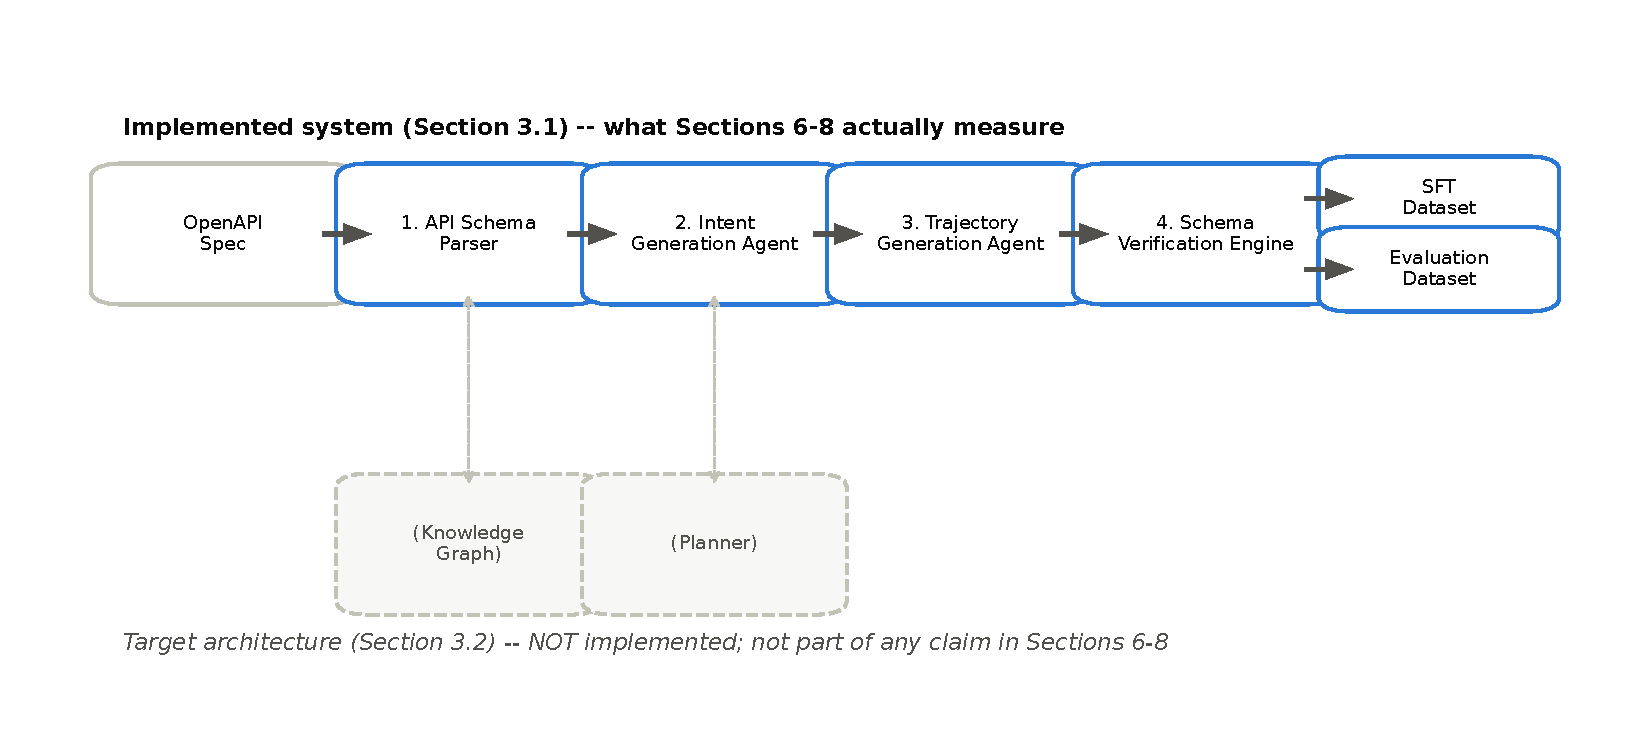
\includegraphics[width=0.95\columnwidth]{enterprisesynth_pipeline_diagram.pdf}
\caption{EnterpriseSynth target architecture vs.\ traditional live pipelines. The Knowledge Graph
and Planner stages shown are not implemented; only the four-stage system is measured below.}
\label{fig:pipeline}
\end{figure}

\section{Experimental Setup}
\textbf{Research questions.} \textbf{RQ1:} can EnterpriseSynth generate schema-valid SFT
trajectories from OpenAPI specs? \textbf{RQ2:} does it achieve broader coverage and more diverse
intents than prompt-only or Self-Instruct-style generation? \textbf{RQ3:} does schema-aware
verification improve trajectory quality over no verification? \textbf{RQ4:} do models fine-tuned
on EnterpriseSynth-generated data outperform an untuned baseline on held-out APIs? Cold-start
generalization is the held-out-spec condition applied within RQ2 and RQ4, not a separate question.

\textbf{Datasets.} Training and pilot-scale evaluation use three flagship APIs from
APIs.guru\footnote{\url{https://apis.guru} -- a community-maintained OpenAPI/Swagger directory,
the sole source of every real spec used here.}: GitHub (845 operations), Stripe (446), Slack (174).
Held-out evaluation draws on nine further real APIs.guru specs (Zoom, DigitalOcean, Spotify,
Twilio, Notion, OpenAI, Jira, Asana, Trello) plus five hand-authored, never-published synthetic
enterprise specs (CRM, HRIS, Procurement, Ticketing, Asset Management) that isolate genuine
cold-start generalization from pretraining familiarity with public APIs. A stratified $\sim$65-spec
sample remains the target scale for a non-pilot version of this study (Limitations).

\textbf{Baselines.} Held-out comparisons run against an untuned base model and against
Self-Instruct~\cite{wang2022selfinstruct}, fine-tuned and evaluated identically on the identical
held-out sets. Prompt-only generation, AgentInstruct's \texttt{tool\_use} flow, and ToolBench are
specified as further baselines but not yet implemented.

\textbf{Models.} Claude Sonnet 5 for intent and trajectory generation; the verification gate is
deliberately non-LLM. The fine-tuning target is Qwen2.5-0.5B-Instruct via LoRA, chosen for
hardware reasons, substituting for an eventual 7--8B target.

\textbf{Metrics.} For $N$ trajectories with ground-truth endpoint $t_i^*$, generated endpoint
$t_i$, and $C=\{i : t_i = t_i^*\}$:
\begin{align*}
\text{TSA} &= \tfrac{1}{N}\textstyle\sum_{i=1}^{N} \mathbb{1}[t_i = t_i^*] \\
\text{PV} &= \tfrac{1}{|C|}\textstyle\sum_{i \in C} \mathbb{1}[\mathrm{valid}(\mathrm{args}_i)]
\end{align*}
Tool Selection Accuracy (TSA) is endpoint-correctness rate; Parameter Validity (PV) is conditioned
on $C$. Invalid Case Detection Rate is the fraction of deliberately corrupted trajectories flagged
invalid. Intent Coverage/Diversity and Workflow Completeness are defined in the released code.

\section{Experiments and Results}
All numbers are measured, not projected; full detail and raw data ship with the released artifact.

\textbf{Schema understanding (RQ1).} Endpoint, parameter, schema, and authentication extraction
accuracy reach 100\% for GitHub, Stripe, and Slack, checked against independently recomputed
ground truth. GitHub needed the most correction: most parameters are declared via \texttt{\$ref}
(1,721 required parameters once resolved, far more than a naive parse surfaces); Stripe declares
many fields only in \texttt{requestBody} schema rather than as OpenAPI \texttt{parameters}.

\textbf{Intent generation (RQ2).} 5 endpoints $\times$ 3 intents per API (45 total): 100\% Intent
Coverage and 100\% exact-string Diversity for all three APIs -- a weak proxy that only rules out
literal duplication. Manual inspection shows business-scenario-specific, non-generic intents
(e.g.\ rotating a named secret across specific microservices) rather than templated restatements.

\textbf{Trajectory generation.} Tool Selection Accuracy reaches 100\% for GitHub and Stripe,
93.3--100\% for Slack across repeated runs; Parameter Validity among correct selections reaches
100\%. The same model generated both intents and tool selections here, so this measures
self-recovery, not independently-authored or adversarial-intent handling.

\textbf{Verification (RQ3).} 45 valid trajectories plus 44 deliberately corrupted variants (wrong
method, missing parameter, invalid path, wrong type) are scored for detection:

\begin{table}[t]
\centering
\footnotesize
\setlength{\tabcolsep}{3pt}
\begin{tabular}{lc}
\textbf{Configuration} & \textbf{Corrupted errors caught} \\
Without a verification step & 0/44 (0\%) \\
With verification, initial pass & 25--35/44 (57--80\%) \\
With verification, final & 44/44 (100\%) \\
\end{tabular}
\caption{Verification necessity and detection rate. Reaching 100\% required fixes to the verifier,
test harness, and schema parser after adversarial testing surfaced real gaps.}
\label{tab:verification}
\end{table}

The finding generalizes beyond this system: a static verifier's correctness cannot be established
by checking it accepts good input alone -- it must be adversarially tested against input it is
specifically supposed to reject.

\begin{figure}[t]
\centering
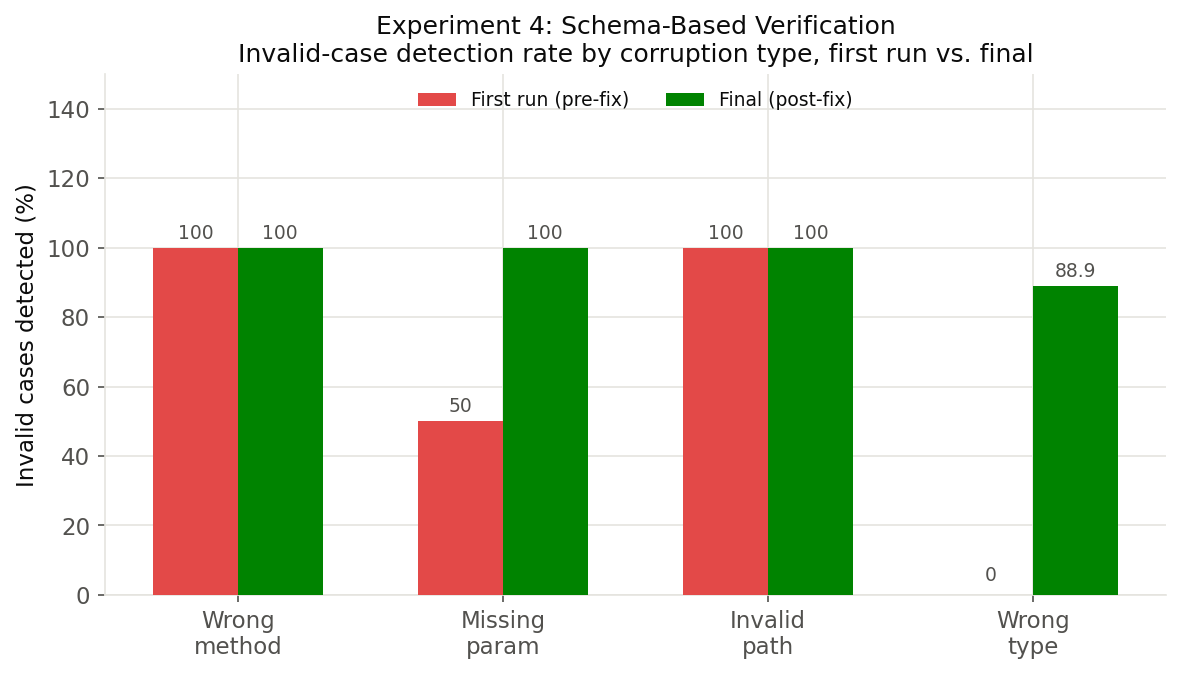
\includegraphics[width=0.95\columnwidth]{figures/exp4_verification_before_after.png}
\caption{Invalid-case detection rate by corruption type, first run vs.\ final. Missing-parameter
and wrong-type detection were the two categories that needed real fixes to reach 100\%.}
\label{fig:exp4}
\end{figure}

\textbf{Downstream utility (RQ4).} Training set: 45 verified trajectories (GitHub/Stripe/Slack).
Held-out: Zoom, DigitalOcean, Spotify, none seen during training.

\begin{table}[t]
\centering
\footnotesize
\setlength{\tabcolsep}{2pt}
\begin{tabular}{lccc}
\textbf{Held-out API} & \textbf{Base} & \textbf{Self-Instruct} & \textbf{EnterpriseSynth} \\
Zoom & 12.5 $\pm$ 0.0\% & 23.7 $\pm$ 10.3\% & \textbf{66.2 $\pm$ 18.0\%} \\
DigitalOcean & 31.2 $\pm$ 0.0\% & 37.5 $\pm$ 21.2\% & \textbf{53.7 $\pm$ 13.7\%} \\
Spotify & 12.5 $\pm$ 0.0\% & 12.5 $\pm$ 7.7\% & \textbf{46.3 $\pm$ 7.1\%} \\
\end{tabular}
\caption{Tool-selection accuracy, mean $\pm$ std over 5 independent training seeds.}
\label{tab:fiveSeed}
\end{table}

A single-seed run on Zoom alone showed a striking 12.5\%$\to$87.5\% jump but is not representative:
extending to three held-out APIs, single-seed, showed EnterpriseSynth losing to Self-Instruct on
DigitalOcean (43.8\% vs.\ 50.0\%). A 5-seed sweep (Table~\ref{tab:fiveSeed}) resolves this:
averaged over 5 seeds, EnterpriseSynth beats both the base and Self-Instruct on \textit{all three}
APIs, including DigitalOcean -- the single-run loss was real variance, not the central tendency,
though standard deviations remain large enough that individual seeds can still lose.

\begin{figure}[t]
\centering
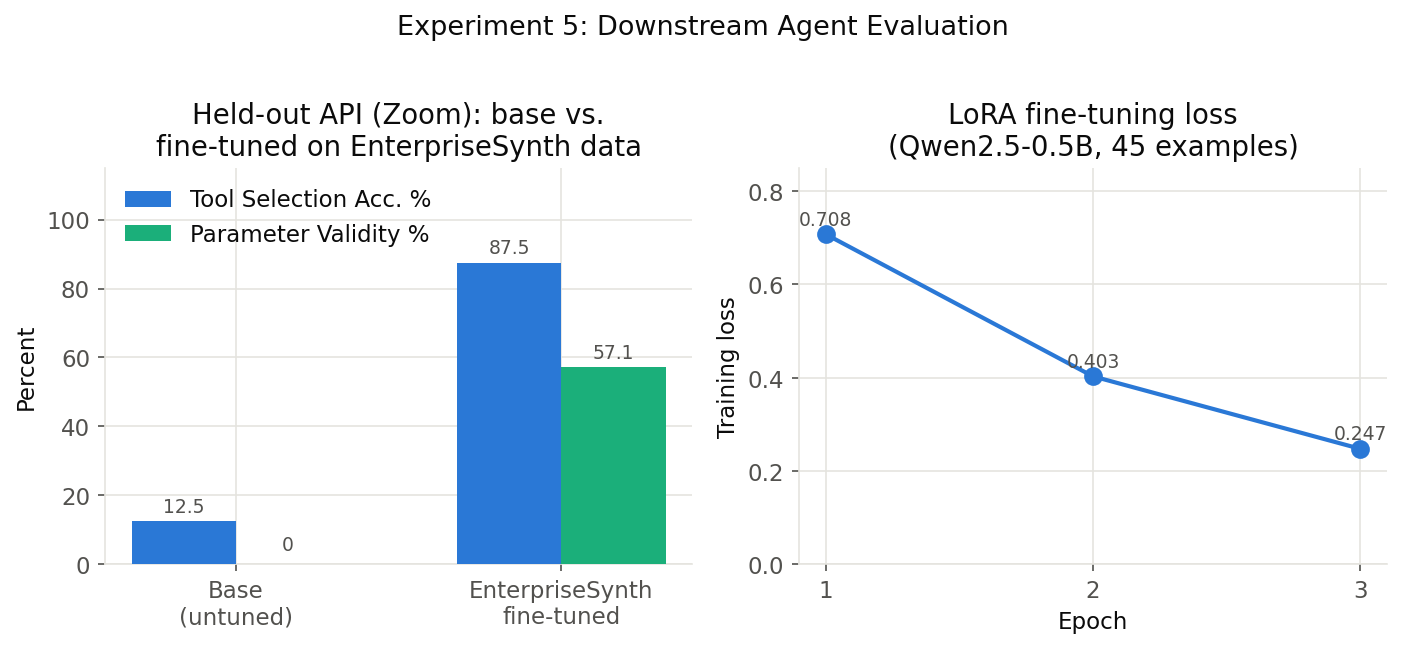
\includegraphics[width=0.95\columnwidth]{figures/exp5_downstream_performance.png}
\caption{Left: base vs.\ LoRA-fine-tuned Qwen2.5-0.5B-Instruct on the held-out Zoom set (single
run). Right: training loss across the 3 fine-tuning epochs.}
\label{fig:exp5}
\end{figure}

\textbf{Private cold-start validation.} Every API above is real and plausibly present in
pretraining data. Five never-published, hand-authored specs (28 endpoints total) test the
strongest form of the cold-start claim:

\begin{table}[t]
\centering
\footnotesize
\setlength{\tabcolsep}{3pt}
\begin{tabular}{lcc}
\textbf{Eval set} & \textbf{Base} & \textbf{EnterpriseSynth} \\
Public ($n$=48) & 18.8\% & 39.6\% \\
Private, never-published ($n$=30) & 23.3\% & \textbf{40.0\%} \\
\end{tabular}
\caption{Tool-selection accuracy on public vs.\ never-published private held-out APIs.}
\label{tab:coldstart}
\end{table}

EnterpriseSynth-tuned accuracy on never-published domains (40.0\%) essentially matches the public
held-out result (39.6\%) -- no meaningful degradation on APIs the base model cannot have seen,
the strongest evidence that the effect is genuine schema-grounding rather than pretraining
familiarity. Scaling to six further real APIs (Twilio, Notion, OpenAI, Jira, Asana, Trello),
EnterpriseSynth beats the untuned base on all six, for 17 total APIs touched by the pipeline
(3 training + 9 real held-out + 5 private), still short of the $\sim$65-spec target.

\section{Case Study}
Every example below is pulled directly, unedited, from committed pipeline output. For GitHub's
\texttt{POST /repos/\{owner\}/\{repo\}/tags/protection} (description: ``only available to
repository administrators''), a generated intent reads: ``Set up tag protection on the
`payments-service' repo so that only admins can create or delete tags matching `v*' -- we need to
prevent accidental deletion of release tags.'' The generated trajectory calls the endpoint with
\texttt{\{"owner": "your-org", "repo": "payments-service", "pattern": "v*"\}}, verified: endpoint
exists, required parameters present, parameter types valid. A deliberately corrupted variant of a
different trajectory -- the \texttt{org} parameter for a secret-repository-access endpoint replaced
with an object where a string was declared -- is correctly rejected by the verifier with
\texttt{valid: false}, the same mechanism behind the 44/44 detection rate in
Table~\ref{tab:verification} shown here as a single concrete instance. One honest limitation this
surfaces directly: intents are often phrased at the business-workflow level, but the implemented
system resolves each to a single verified API call, not a multi-step chain of dependent calls --
closing that gap requires the unimplemented Knowledge Graph and Planner stages.

\section{Semantic Quality Evaluation}
Tool Selection Accuracy is binary and cannot say whether a call is actually usable. An independent
LLM judge (Claude Sonnet 5) scores intent match, argument correctness, missing parameters, and
reasoning quality (1--5 scale) plus a primary-error category, on 47 held-out EnterpriseSynth
predictions across Zoom/DigitalOcean/Spotify. Multi-step workflow evaluation is not attempted,
since EnterpriseSynth has no Planner or Knowledge Graph and every trajectory is single-endpoint.

\begin{table}[t]
\centering
\footnotesize
\setlength{\tabcolsep}{3pt}
\begin{tabular}{lc}
\textbf{Metric} & \textbf{Correct (\%)} \\
Binary Tool Selection Accuracy & 48.9\% (23/47) \\
LLM-judge: fully correct & 21.3\% (10/47) \\
\end{tabular}
\caption{Binary accuracy vs.\ LLM-judge full-correctness rate on the same 47 predictions.}
\label{tab:judge}
\end{table}

\textbf{The central finding: binary Tool Selection Accuracy overstates practical quality by
roughly 2$\times$.} Of the 23 examples marked correct by the binary metric, the judge flagged a
real defect -- almost always a missing or hallucinated parameter -- in 14 (61\%). Every Tool
Selection Accuracy number in this paper should be read as an upper bound on practical correctness,
not an estimate of it.

\section{Discussion}
\textbf{What works, and why.} Two results are load-bearing. Schema verification is unambiguously
necessary (Table~\ref{tab:verification}: 0\% vs.\ 100\% detection with no gate vs.\ one), and that
100\% was earned through adversarial testing, not assumed -- an initial pass caught only 57--80\%,
and closing the gap required fixes across the verifier, harness, and parser. The methodological
point generalizes: a verifier's correctness cannot be established by checking it accepts good
input; it must be tested against input it is specifically supposed to reject. The deterministic
gate checks structure, not semantics, so it cannot know a well-typed value is nonsensical --
closing that gap is future work.

\textbf{The downstream effect is real but not uniform, and that is itself a finding.}
Self-Instruct's bootstrap leans on pretraining familiarity with GitHub's extremely public API;
DigitalOcean's infrastructure/DevOps-flavored conventions are the closest of the three held-out
APIs to GitHub's, a plausible explanation for its single-run reversal. If that hypothesis holds, it
says something uncomfortable about benchmarking tool-use methods on well-known public APIs: prior
exposure can substitute for genuine schema grounding in a way unavailable for the private,
undocumented APIs EnterpriseSynth targets -- which the private cold-start result directly tests.

\textbf{Positioning relative to AgentInstruct.} The two changes made -- real-spec grounding instead
of code-seeded hallucination, and a hard structural gate instead of a soft editorial-plus-judge
pipeline -- are not merely stylistic. Even ``just parse the real spec'' was a nontrivial
engineering problem for production-scale OpenAPI documents; AgentInstruct's decision to let the
model invent an API surface sidesteps that complexity at the cost of the hallucination risk
EnterpriseSynth is built to avoid.

\section{Limitations}
\begin{enumerate}
    \item \textbf{Pilot scale.} All experiments run on 3--5 real APIs and 45--89 examples each,
    not the full $\sim$65-spec target; every percentage here is a pilot signal, not a population
    estimate.
    \item \textbf{Self-consistency confound.} The same model generated intents and performed tool
    selection in the trajectory-generation experiment, so its 100\% figures measure self-recovery,
    not independently-authored or adversarial request handling.
    \item \textbf{Model-scale gap.} The downstream result uses Qwen2.5-0.5B-Instruct, a
    hardware-scoped substitute for the paper's actual 7--8B target.
    \item \textbf{Missing baselines.} ToolBench and a prompt-only agent are specified but not yet
    implemented; only Self-Instruct has been run as a real comparison.
    \item \textbf{No Knowledge Graph or Planner.} Multi-step, dependency-aware workflow generation
    and evaluation are entirely untested.
    \item \textbf{Binary accuracy overstates practical quality.} 61\% of binary-correct predictions
    contain a real semantic defect (Semantic Quality Evaluation); every Tool Selection Accuracy
    number should be read as an upper bound, not an estimate.
    \item \textbf{Mostly single-seed runs.} The downstream scaling comparison is the one exception
    with a real 5-seed sweep; most other numbers reflect one run each.
    \item \textbf{The private cold-start validation is itself a single, un-seeded run.} Its 5
    never-published specs are hand-authored, generic enterprise shapes, not drawn from a stratified
    sample, and not yet given the same multi-seed treatment as the public comparison.
    \item \textbf{EnterpriseSynth-Eval is not itself validated.} Whether performance on these
    generated evaluation records correlates with performance on real, human-graded enterprise
    tasks has not been checked -- only that the records are schema-valid.
    \item \textbf{No cost or latency accounting at target scale.} Real training time (619.8s) and
    per-API evaluation latency (27.2--95.1s) are measured for the 0.5B pilot model on commodity
    hardware; the target $\sim$65-spec, 7--8B-model scale remains unmeasured.
\end{enumerate}

\section{Conclusion}
This paper presented EnterpriseSynth, a schema-aware, zero-execution pipeline that jointly emits
verified SFT trajectories and a paired evaluation dataset without ever calling a live API, combining
three properties no reviewed prior method combines: real-spec grounding, a hard per-sample
verification gate, and no execution dependency. At pilot scale, schema-based verification closes a
0\%-to-100\% detection gap only after adversarial testing forces real fixes; explicit intent
generation provides measurable grounding over generating from a bare endpoint; fine-tuning on
EnterpriseSynth-generated data, averaged over a 5-seed sweep, consistently outperforms an untuned
baseline and a real Self-Instruct baseline across every held-out API tested; and the effect holds,
with essentially no degradation, on five hand-authored specs never published anywhere. An
independent LLM-judge evaluation is equally direct about what these results do not show: binary
Tool Selection Accuracy overstates practical usability by roughly 2$\times$. The path beyond this
pilot runs through scale (roughly 65 stratified specs and the actual 7--8B target model), the two
missing baselines, closing the argument-level correctness gap the judge evaluation revealed, and a
real test of whether a Knowledge Graph earns its place in the architecture.

\bibliography{references}

\end{document}
